\graphicspath{{introduction/fig/}}

\chapter{Introduction}
\label{chap:introduction}

\section{Background}
In South Africa, millions of commuters use taxis frequently and depend on them for all of their mobility needs \cite{depttransport2023}.\\
The South African government has recognised the impact of taxi emissions on air quality and has taken steps to address the issue. In 2006, the government gazetted regulations that required taxi operators to convert their vehicles to run on cleaner fuels, such as liquefied petroleum gas (LPG), compressed natural gas (CNG), or diesel with lower sulphur content\cite{2007Comparison}. 

\begin{figure}[!htb]
	\minipage{0.32\textwidth}%
	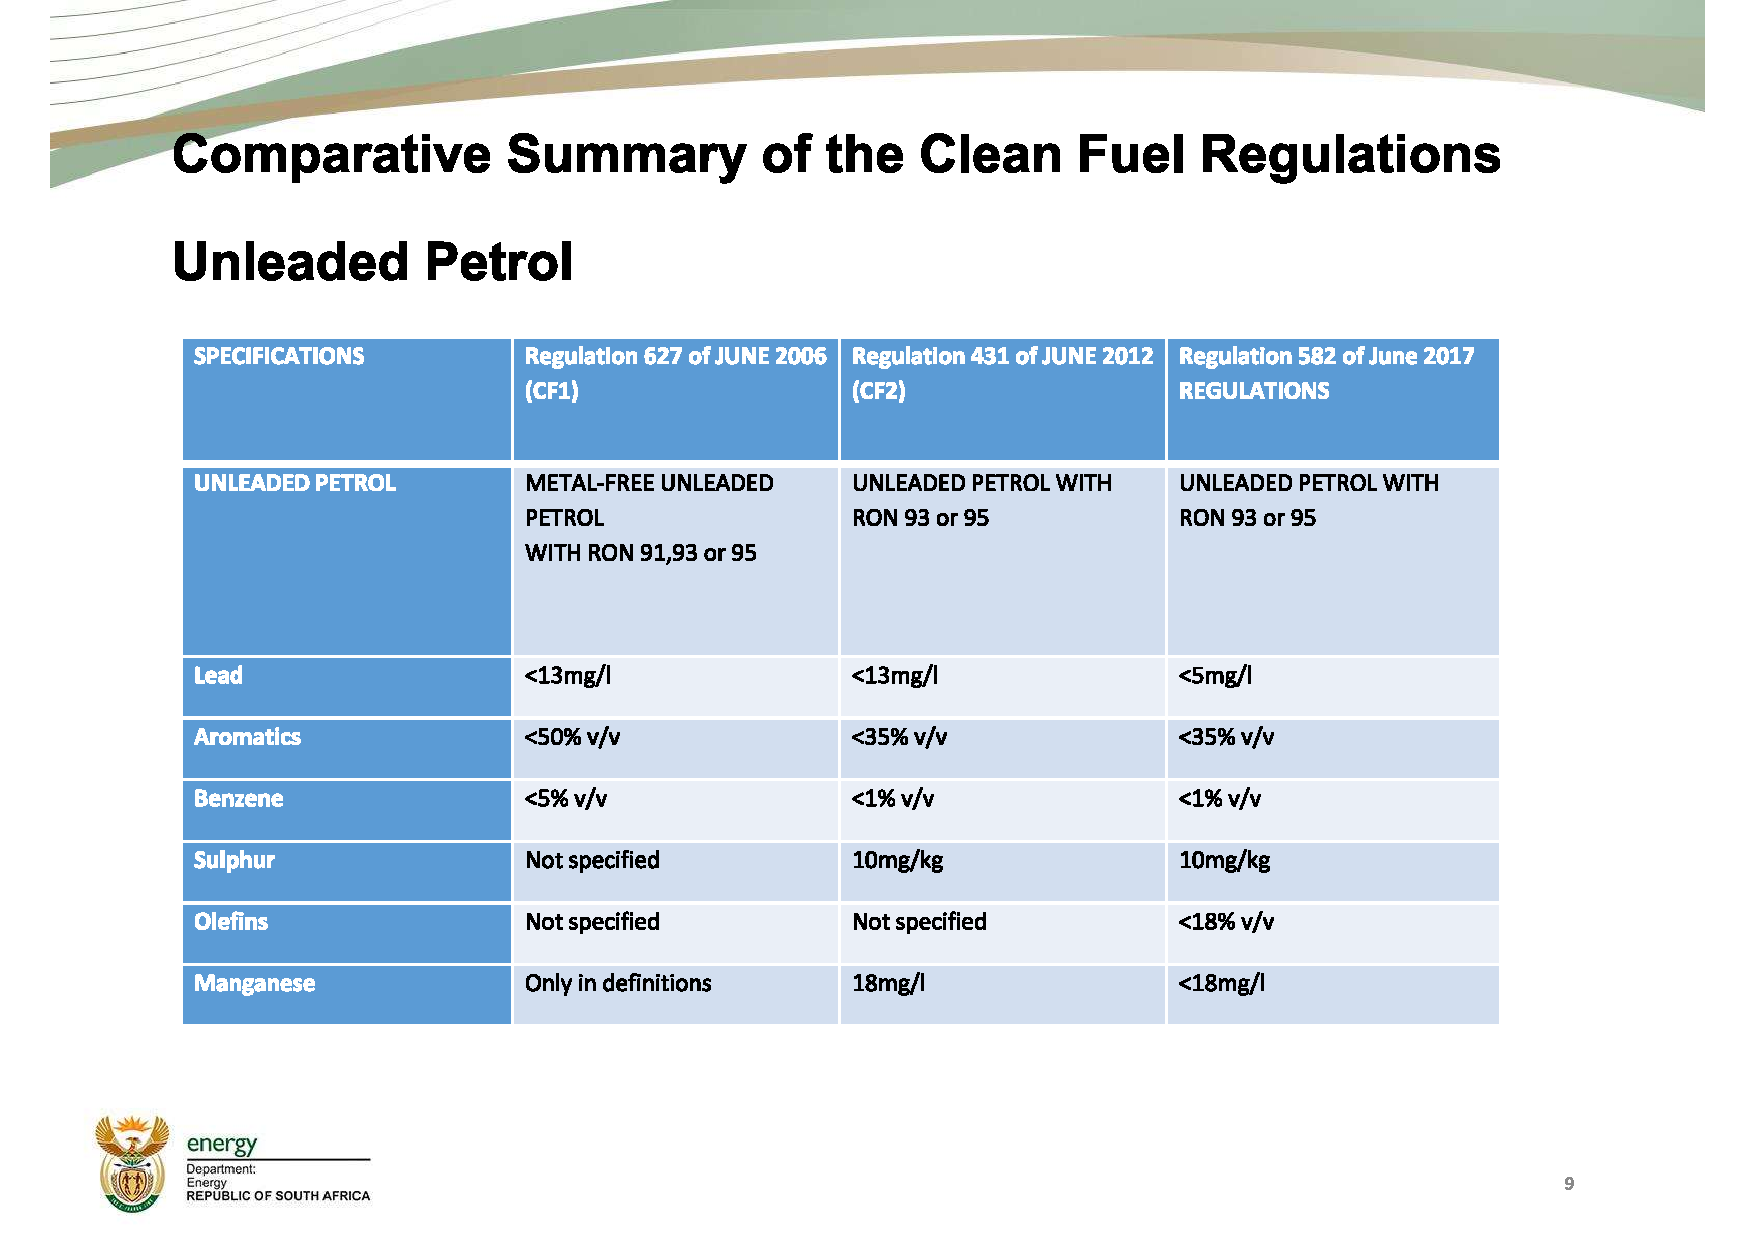
\includegraphics[width=\linewidth]{introduction/fig/page1Comp.pdf}
	\caption{Unleaded\cite{2007Comparison}}\label{fig:fig1}
	\endminipage\hfill
	\minipage{0.32\textwidth}%
	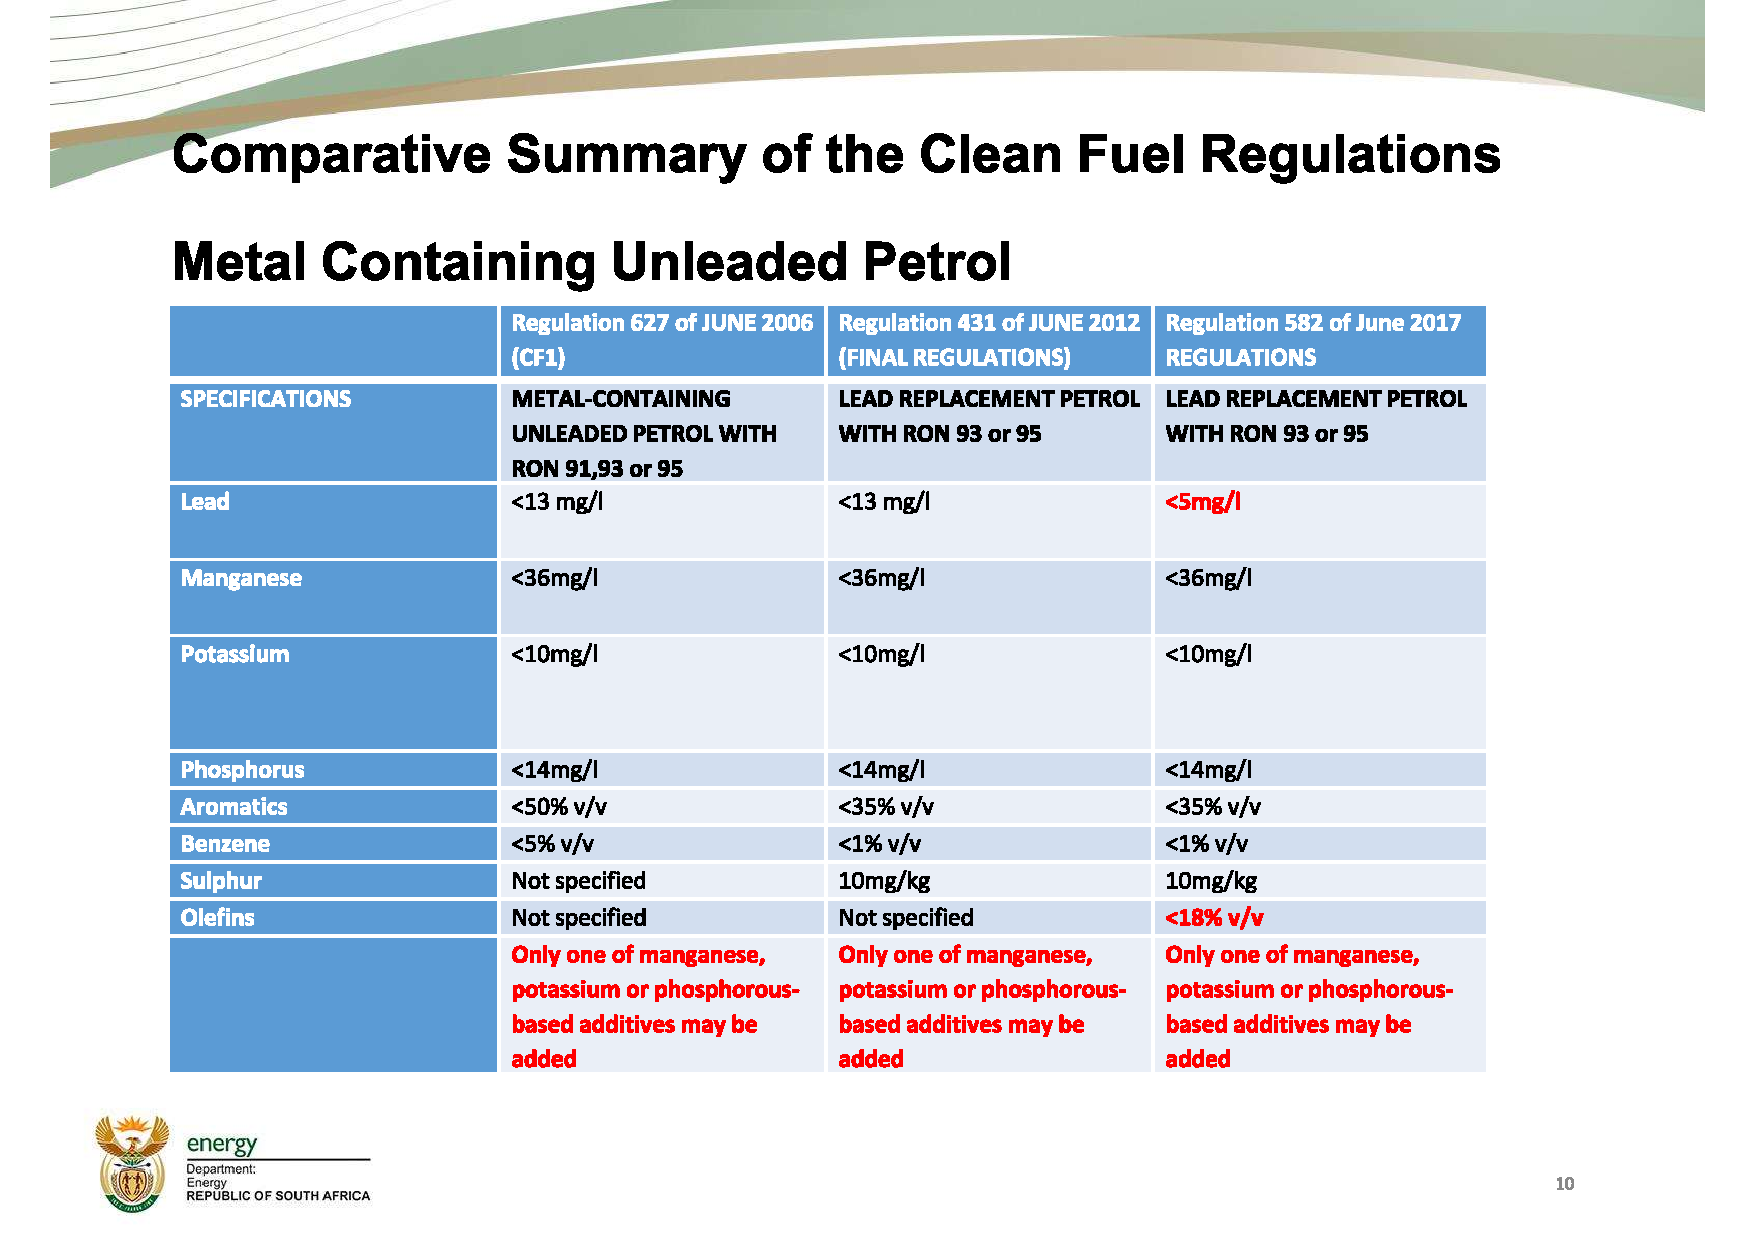
\includegraphics[width=\linewidth]{introduction/fig/page2Comp.pdf}
	\caption{Metal+ Unleaded\cite{2007Comparison}}\label{fig:fig2}
	\endminipage\hfill
	\minipage{0.32\textwidth}%
	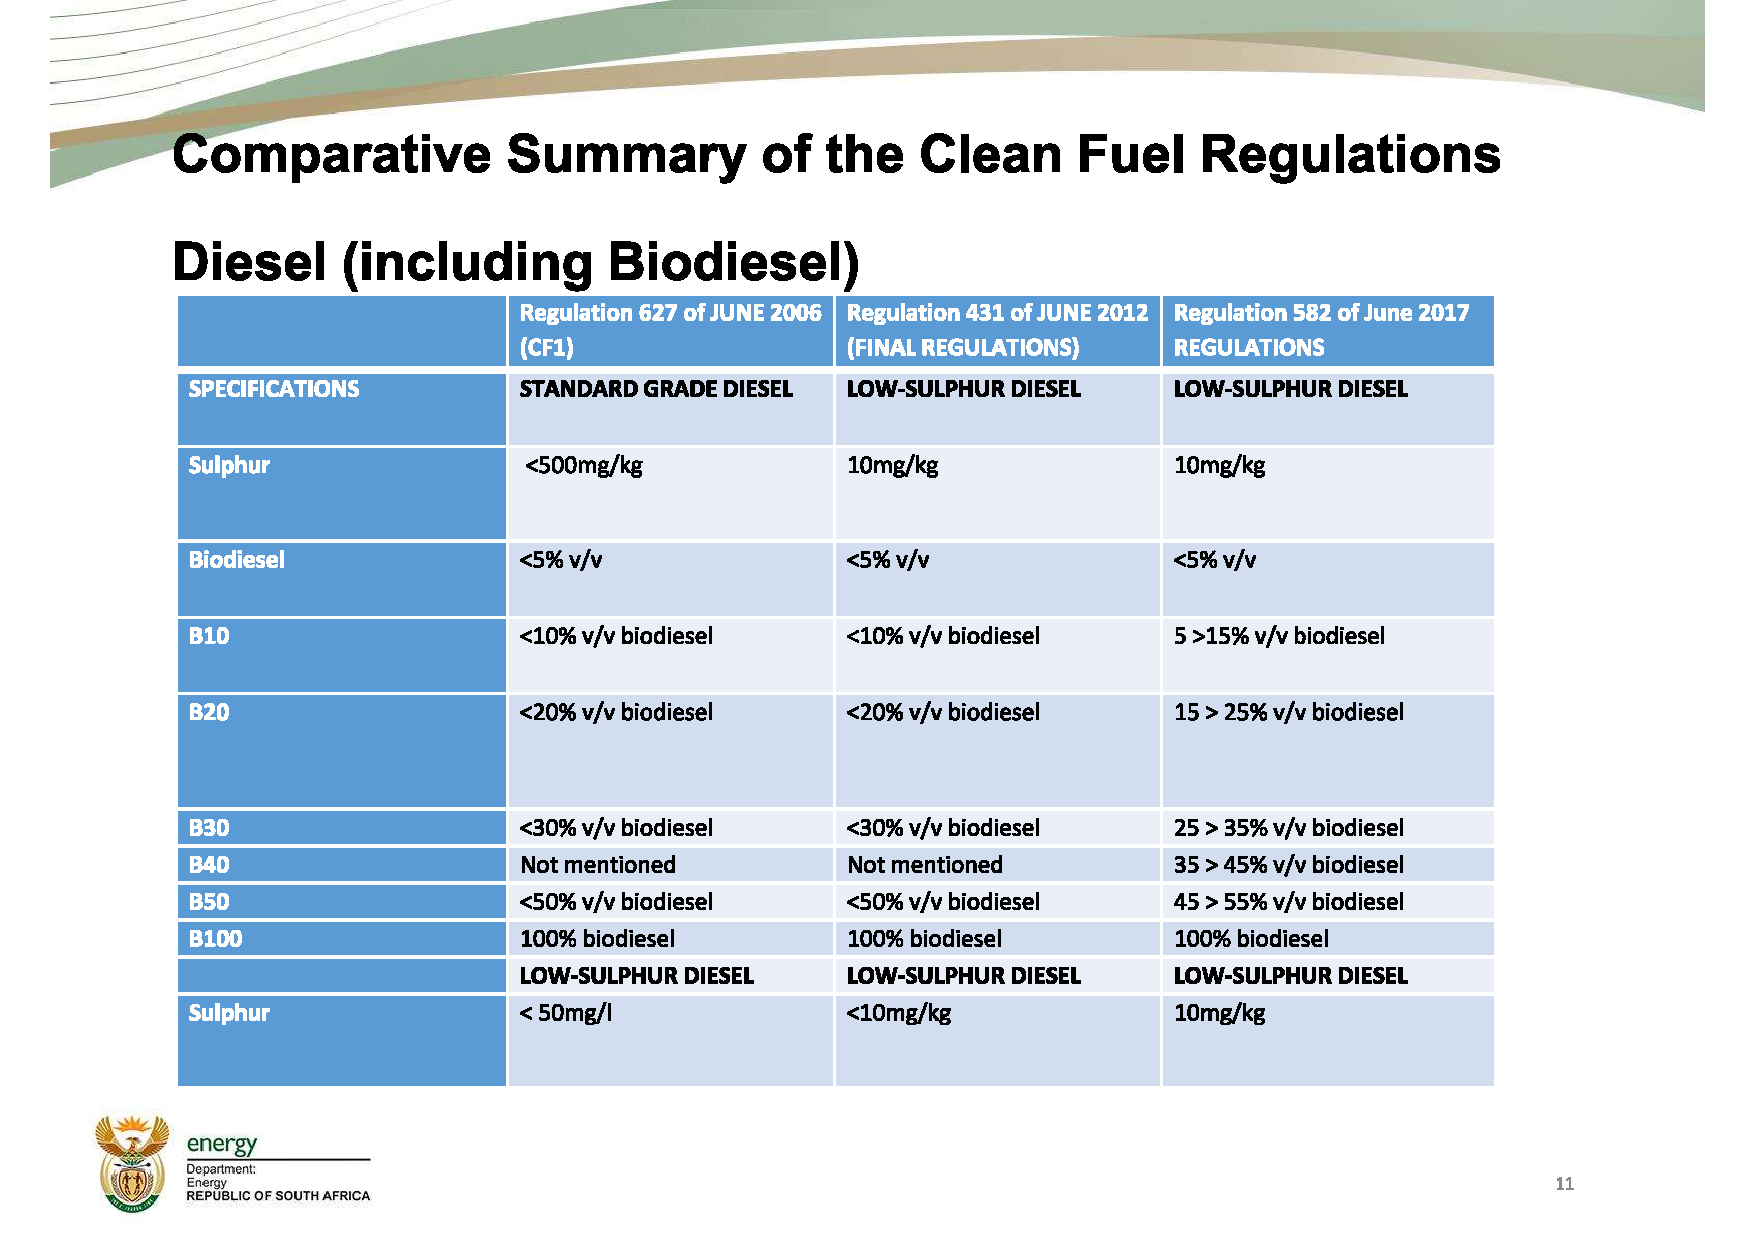
\includegraphics[width=\linewidth]{introduction/fig/page3Comp.pdf}
	\caption{Diesel\cite{2007Comparison}}\label{fig:fig3}
	\endminipage
	%\text{Charts provided by \cite{2007Comparison}}
\end{figure}

\noindent
As seen in Figures \ref{fig:fig1}, \ref{fig:fig2} and \ref{fig:fig3} South Africa's regulations on cleaner fuels are updated every five to six years. Cleaner fuels produce less greenhouse emissions. The implementation of these regulations has been slow and often poorly regulated \cite{newcleanfuelstandards}, resulting in continued poor air quality in many areas.

\noindent
The main sources of air pollution in South Africa are industrial activities, power generation, vehicle emissions, biomass burning, and domestic fuel use \cite{Bylaws2023}. Among these sources, vehicle emissions are particularly relevant for taxi commuters, who are exposed to high levels of pollutants such as particulate matter (PM), nitrogen oxides (NOx), carbon monoxide (CO), and volatile organic compounds (VOCs) \cite{Venter2018}. These pollutants can have adverse effects on respiratory, cardiovascular, neurological, and immune systems, as well as increase the risk of cancer and premature death \cite{WHO2016}.

%Instead of using expensive and inconvenient formal public transportation like buses and trains, they offer an accessible and affordable substitute.

{\color{red} \huge Need to rewrite}
\section{Problem Statement}
Despite the popularity and importance of taxis in South Africa, there is a lack of research on the air quality inside these vehicles and at taxi ranks. 
Air quality is a crucial factor for human health and well-being, especially for commuters who spend long hours in taxis exposed to various pollutants.
Moreover, taxi emissions contribute to the overall air pollution in crowded spaces (in this case taxi ranks), which affects the environment and the quality of life of the passers by. The closest studies are concerning single cab taxis\cite{insidetaxismall}, road based pollution\cite{taxiNetwork} and general pollution\cite{Environmentalimpact}.
There is a need for a study on the air quality in taxis and taxi ranks and its impacts on human health and the environment, this report aims to provide a means to that end.

\section{Objectives}
The objective of the study are as follows:
\begin{itemize}
	\item To design a device to measure the levels of:
		\begin{itemize}
			\item CO2
			\item VOC
			\item NOx
			\item Particulate Matter
		\end{itemize}
	%	 CO2, VOC, particulate matter and NOx
 both inside taxis and in taxi ranks.
%	\item Identify the primary sources of air pollution in taxi ranks and within taxis and evaluate the impact of environmental factors, such as traffic congestion and weather conditions(optional- time limited).
	\item To investigate the potential health risks associated with exposure to air pollution in taxi ranks and within taxis, particularly for passengers, drivers and potential third parties.
%	\item To evaluate the effectiveness of current measures in place to reduce air pollution from taxis, such as emission standards and regulations.
	\item Develop hardware that measures the above-mentioned.
	\item Develop software/firmware that integrates the hardware and makes it user accessible.
%	\item Propose potential strategies to mitigate the impact of  from taxis on public health and the environment such as implementing new technologies.
\end{itemize}


%\section{Summary of Work}??


\section{Scope}
The scope of the project encompasses only the following:

\begin{itemize}
	\item Design of base station and satellite module
	\item Design of communication network for satellite module and base station as well as data storage and backup
	%\item Deployment of sensor and network
%	\item Analysis of data gathered
	\item Hardware development
	\item Software development
	\item Test of Hardware and Software elements
\end{itemize}

\section{Report Overview}%Roadmap


{\color{red}  \LARGE NEED TO DO THIS}








%This is some section with two table in it: Table~\ref{tbl:exemplars} and Table~\ref{tbl:abx_speaker}.

%	\begin{table}[!h]
%	    \mytable
%	    \caption{Performance of the unconstrained segmental Bayesian model on TIDigits1 over iterations in which the reference set is refined.}
%	    \begin{tabularx}{\linewidth}{@{}lCCCCC@{}}
%	        \toprule
%	        Metric     & 1 & 2 & 3 & 4 & 5 \\
%	        \midrule
%	        WER (\%)                        & $35.4$ & $23.5$ & $21.5$ & $21.2$ & $22.9$ \\
%	        Average cluster purity (\%)       & $86.5$ & $89.7$ & $89.2$ & $88.5$ & $86.6$ \\
%	        Word boundary $F$-score (\%)         & $70.6$ & $72.2$ & $71.8$ & $70.9$ & $69.4$ \\
%	        Clusters covering 90\% of data   & 20             & 13 & 13 & 13 & 13 \\
%	        \bottomrule
%	    \end{tabularx}
%	    \label{tbl:exemplars}
%	\end{table}


%\begin{table}[!h]
%    \renewcommand{\arraystretch}{1.1}
%    \centering
%    \caption{A table with an example of using multiple columns.}
%    \begin{tabularx}{0.65\linewidth}{@{}lCCr@{}}
%        \toprule
 %       & \multicolumn{2}{c}{Accuracy (\%)} \\
%        \cmidrule(lr){2-3}
%        Model    & Intermediate & Output & Bitrate\\
%        \midrule
%        Baseline & 27.5         & 26.4   & 116 \\
%        VQ-VAE   & 26.0         & 22.1   & 190 \\
%        CatVAE   & 28.7         & 24.3   & 215 \\
 %    \end{tabularx}
%    \label{tbl:abx_speaker}
%\end{table}

%\newpage

%This is a new page, showing what the page headings looks like, and showing how to refer to a figure like Figure~\ref{fig:cae_siamese}.

%\begin{figure}[!t]
%    \centering
%%     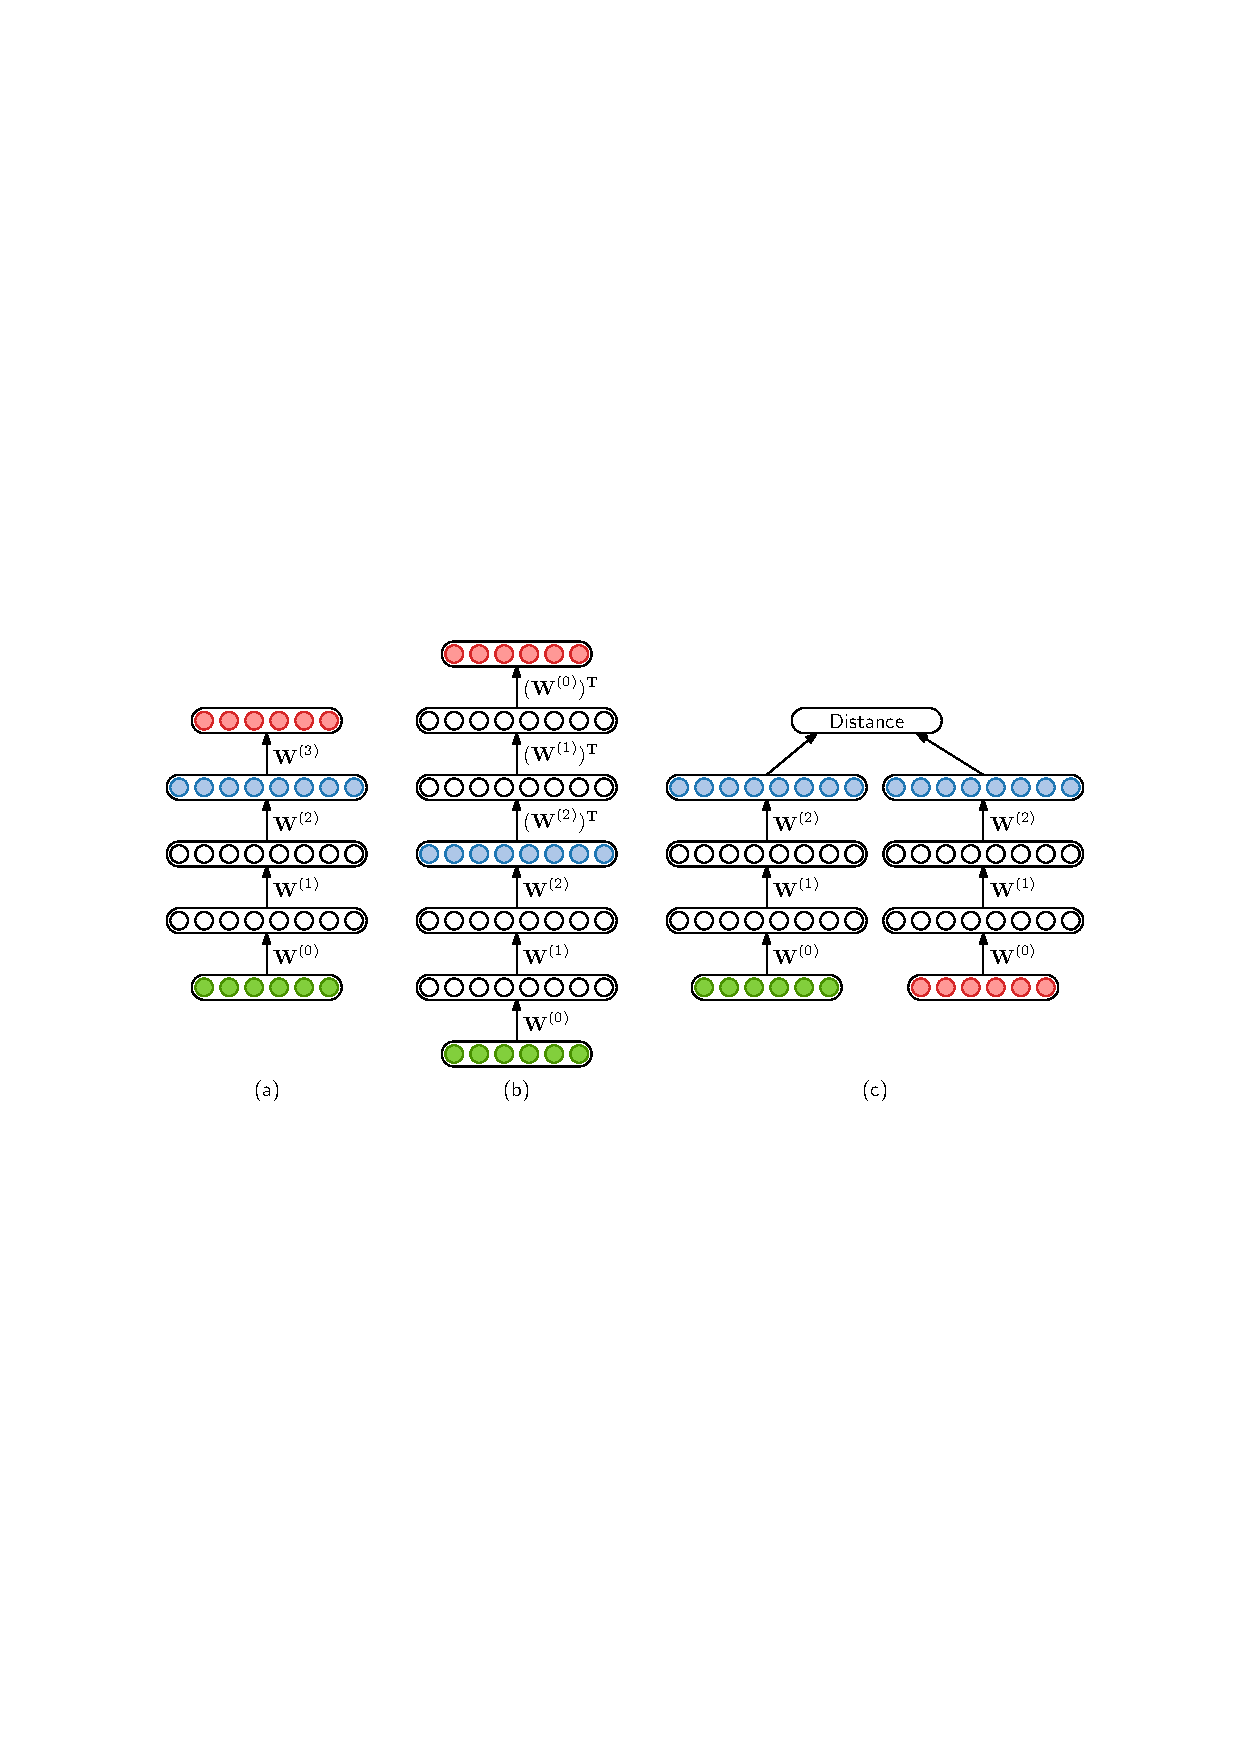
\includegraphics[width=\linewidth]{cae_siamese}
%    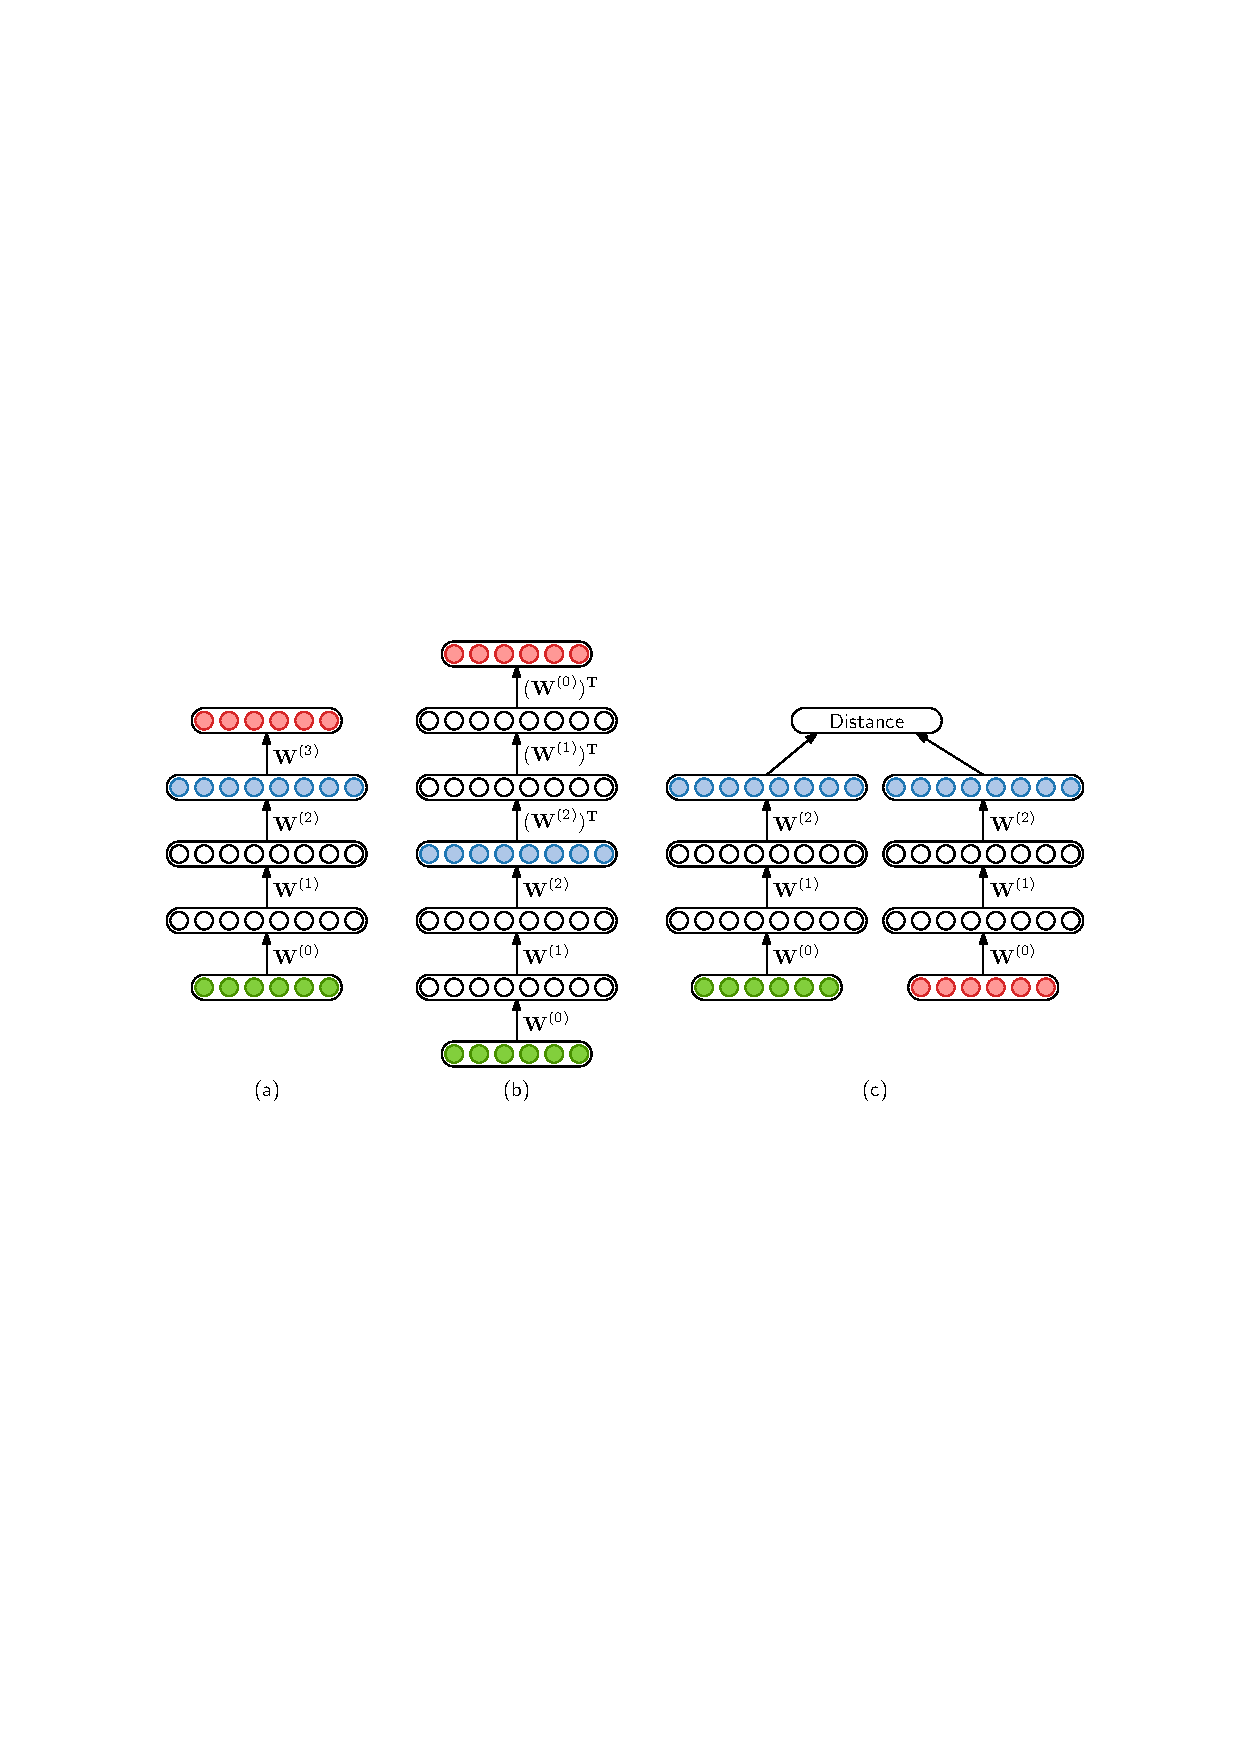
\includegraphics[width=0.918\linewidth]{cae_siamese}
%    \caption[I am the short caption that appears in the list of figures, without references.]{
%    (a) The cAE as used in this chapter. The encoding layer (blue) is chosen based on performance on a development set.
%    (b) The cAE with symmetrical tied weights. The encoding from the middle layer (blue) is always used.
%    (c) The siamese DNN. The cosine distance between aligned frames (green and red) is either minimized or maximized depending on whether the frames belong to the same (discovered) word or not.
%    A cAE can be seen as a type of DNN.
%    }
%    \label{fig:cae_siamese}
%\end{figure}

%
%The following is an example of an equation:
%\begin{equation}
%P(\vec{z} | \vec{\alpha}) = \int_{\vec{\pi}} P(\vec{z} | \vec{\pi}) \, p(\vec{\pi} | \vec{\alpha}) \, \textrm{d} \vec{\pi}
%= \int_{\vec{\pi}} \prod_{k = 1}^K \pi_k^{N_k} \frac{1}{B(\vec{\alpha})} \prod_{k = 1}^K \pi_k^{\alpha_k - 1} \, \textrm{d} \vec{\pi}
%\label{eq:example_equation}
%\end{equation}
%which you can subsequently refer to as~\eqref{eq:example_equation} or Equation~\ref{eq:example_equation}.
%But make sure to consistently use the one or the other (and not mix the two ways of referring to equations).